%% LyX 2.2.3 created this file.  For more info, see http://www.lyx.org/.
%% Do not edit unless you really know what you are doing.
\documentclass[english]{article}
\renewcommand{\familydefault}{\sfdefault}
\usepackage[T1]{fontenc}
\usepackage[latin9]{inputenc}
\usepackage[a4paper]{geometry}
\geometry{verbose,tmargin=2cm,bmargin=2.5cm,lmargin=1cm,rmargin=1cm,headsep=1cm}
\usepackage{graphicx}
\usepackage{wasysym}

\makeatletter

%%%%%%%%%%%%%%%%%%%%%%%%%%%%%% LyX specific LaTeX commands.
%% Because html converters don't know tabularnewline
\providecommand{\tabularnewline}{\\}
%% A simple dot to overcome graphicx limitations
\newcommand{\lyxdot}{.}


\makeatother

\usepackage{babel}
\begin{document}
\date{}

\title{\textbf{\Huge{}Kitchen Kopf (SMD)}}

\maketitle
\maketitle \thispagestyle{empty}
\begin{center}
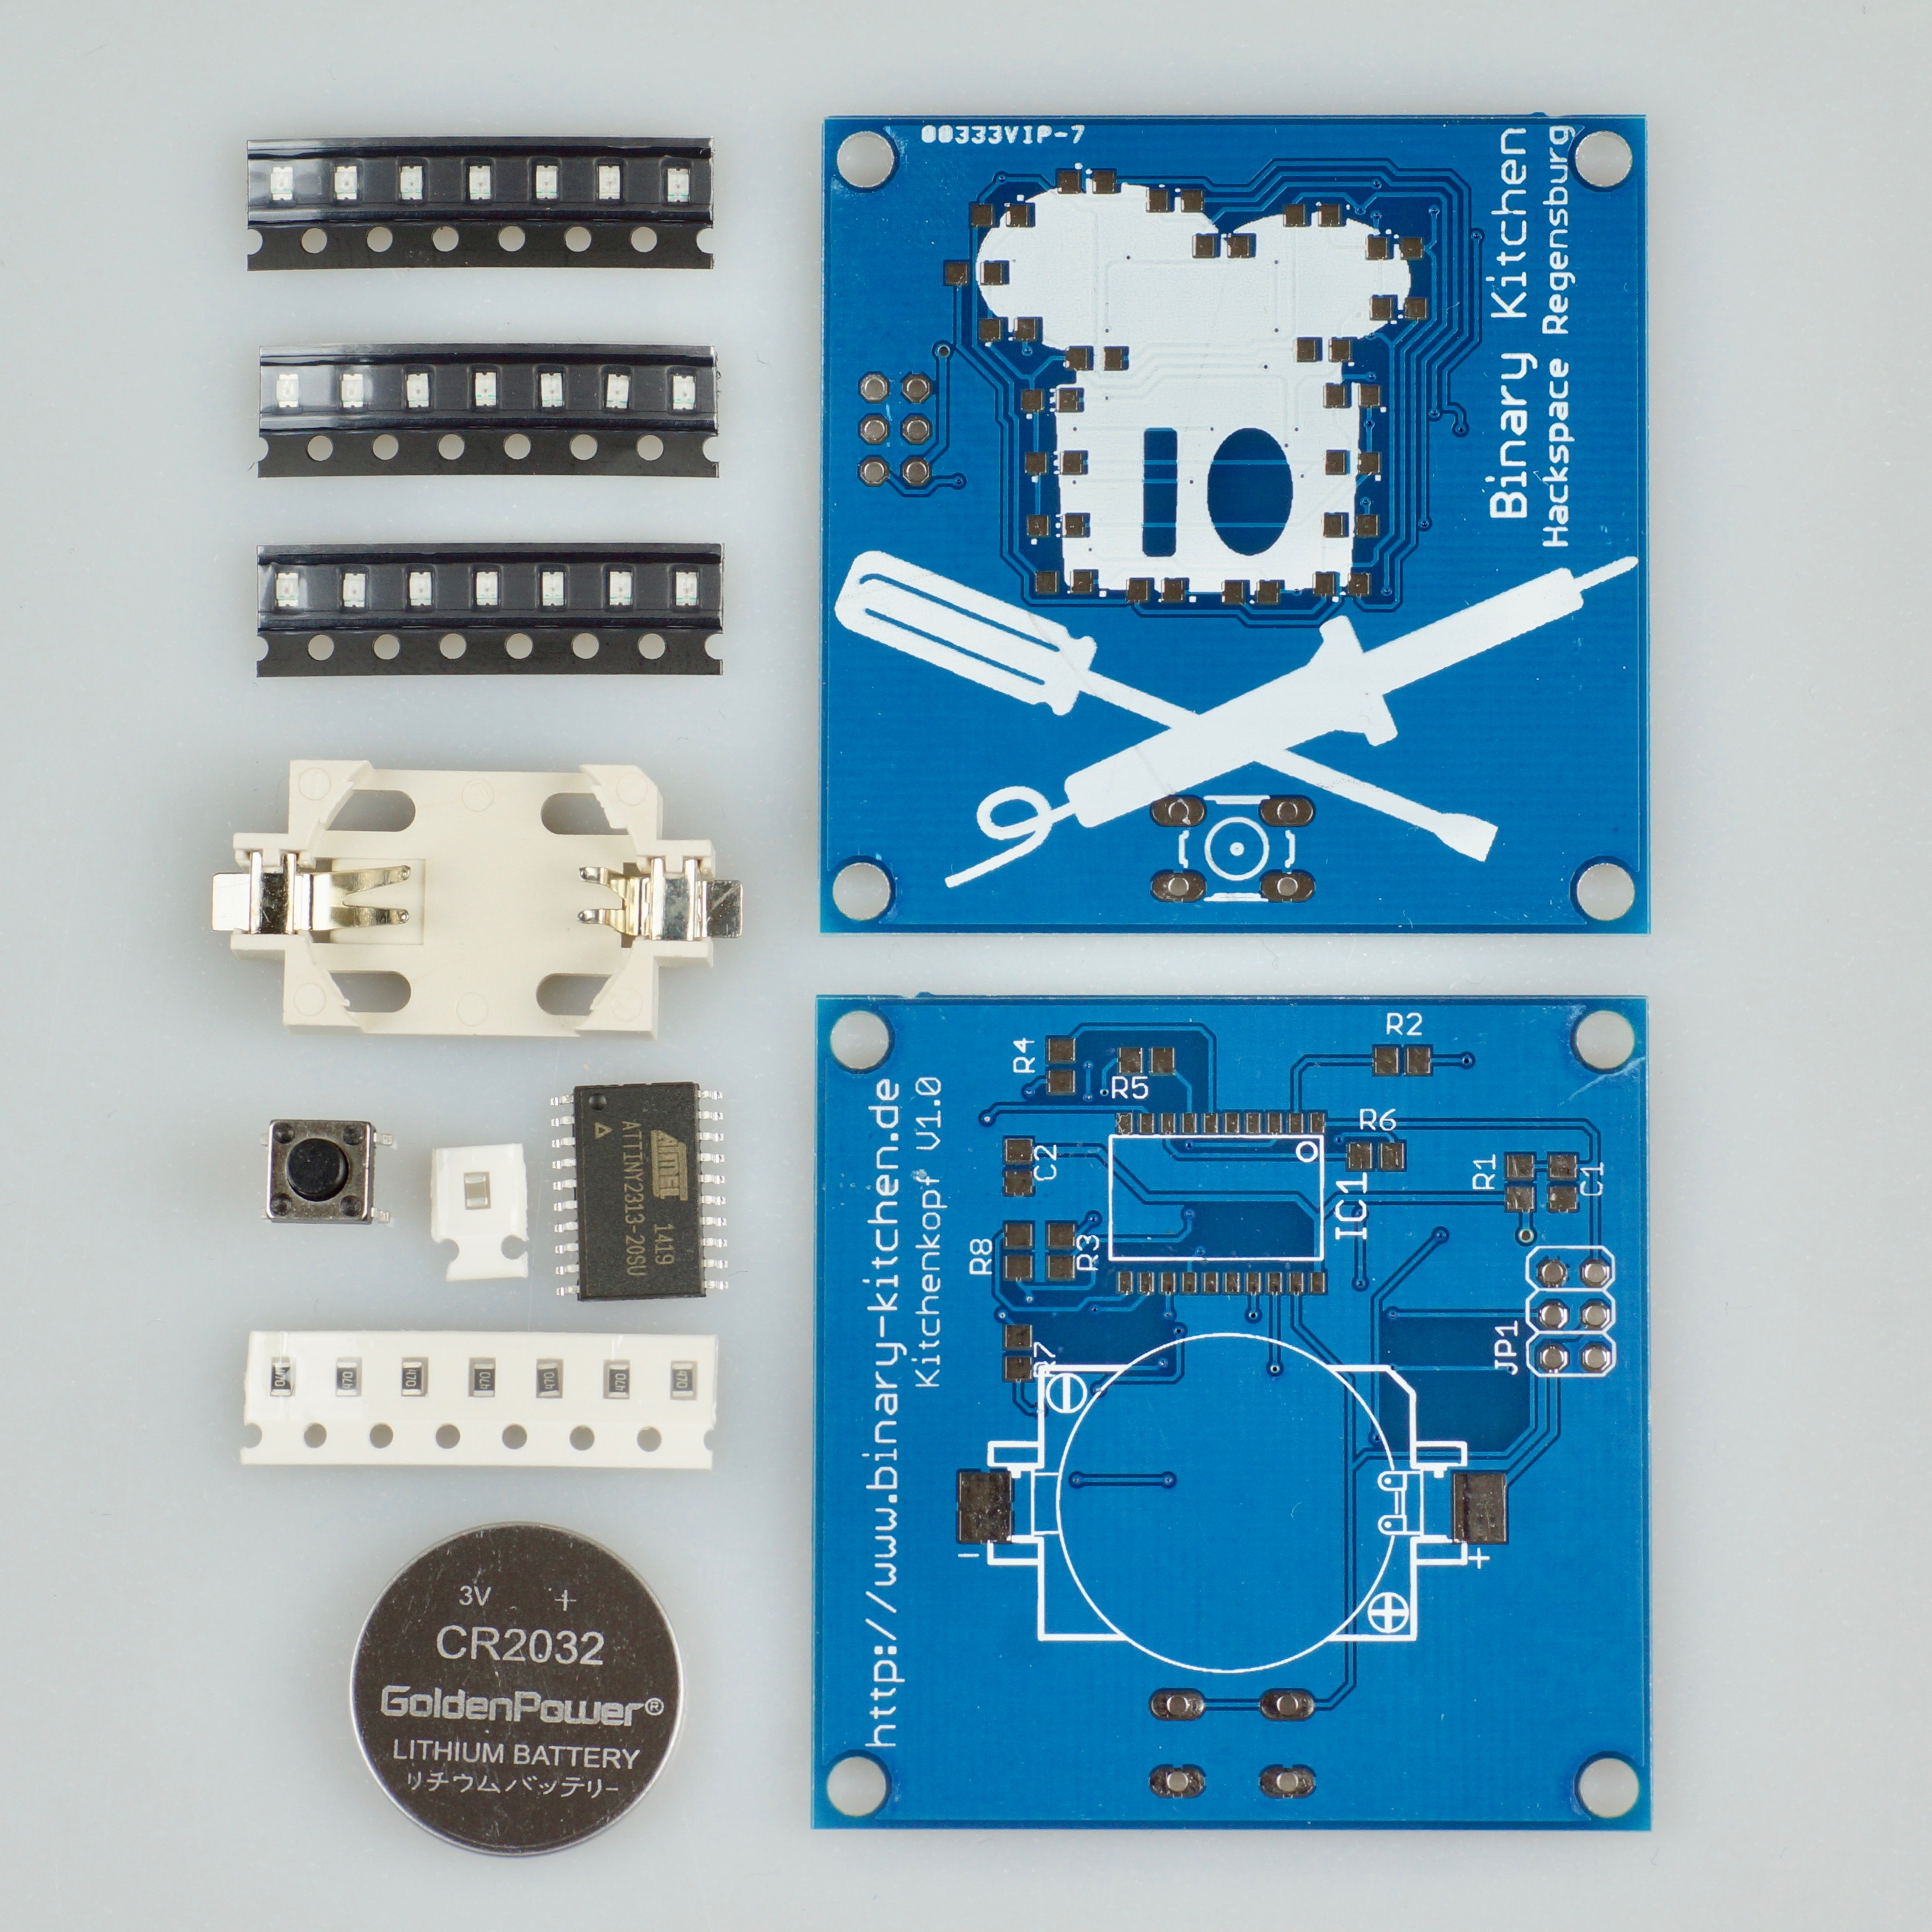
\includegraphics[width=10cm]{images/modified/DSC04829}
\par\end{center}

\vspace{10mm}

\renewcommand{\arraystretch}{1.3}
\begin{center}
\begin{tabular}{llll}
\hline 
Menge & Bezeichnung & Beschreibung & Beschriftung\tabularnewline
\hline 
1 & C2 & Kondensator 100 nF & \tabularnewline
1 & IC2 & Atmel ATTiny 2313A & \tabularnewline
21 & LED1 - LED21 & LED SMD 0805 & \tabularnewline
7 & R2 - R8 & Wiederstand 47 $\Omega$ & 470\tabularnewline
1 & SW1 & Taster & \tabularnewline
1 & BAT1 & Batteriehalter & \tabularnewline
1 &  & Batterie CR2032 & \tabularnewline
1 &  & Platine & \tabularnewline
\hline 
\end{tabular}
\par\end{center}

\begin{center}
\vspace{10mm}
\begin{minipage}[t][1\totalheight][b]{22mm}%
Schwierigkeit:%
\end{minipage}%
\begin{minipage}[t][1\totalheight][b]{25mm}%
{\Large{}\CIRCLE \CIRCLE \CIRCLE \CIRCLE \Circle{}}%
\end{minipage}
\par\end{center}

\vspace{10mm}
\begin{center}
\begin{tabular}{ll}
Anleitung: & v1.0 - CC-BY-SA 4.0 Binary Kitchen e.V.\tabularnewline
Platine: & v1.1 - CC-BY-SA 4.0 Binary Kitchen e.V.\tabularnewline
\end{tabular}
\par\end{center}

\newpage{}
\begin{center}
\rule[0.5ex]{0.9\columnwidth}{1pt}
\par\end{center}

\begin{center}
\begin{minipage}[t][1\totalheight][b]{0.59\columnwidth}%
\begin{enumerate}
\item Vollst�ndigkeit der Bauteile �berpr�fen
\item Platine mit Klebestreifen auf der Unterlage befestigen
\end{enumerate}
%
\end{minipage}\hspace{5mm}%
\begin{minipage}[t][1\totalheight][b]{0.3\columnwidth}%
\begin{flushright}
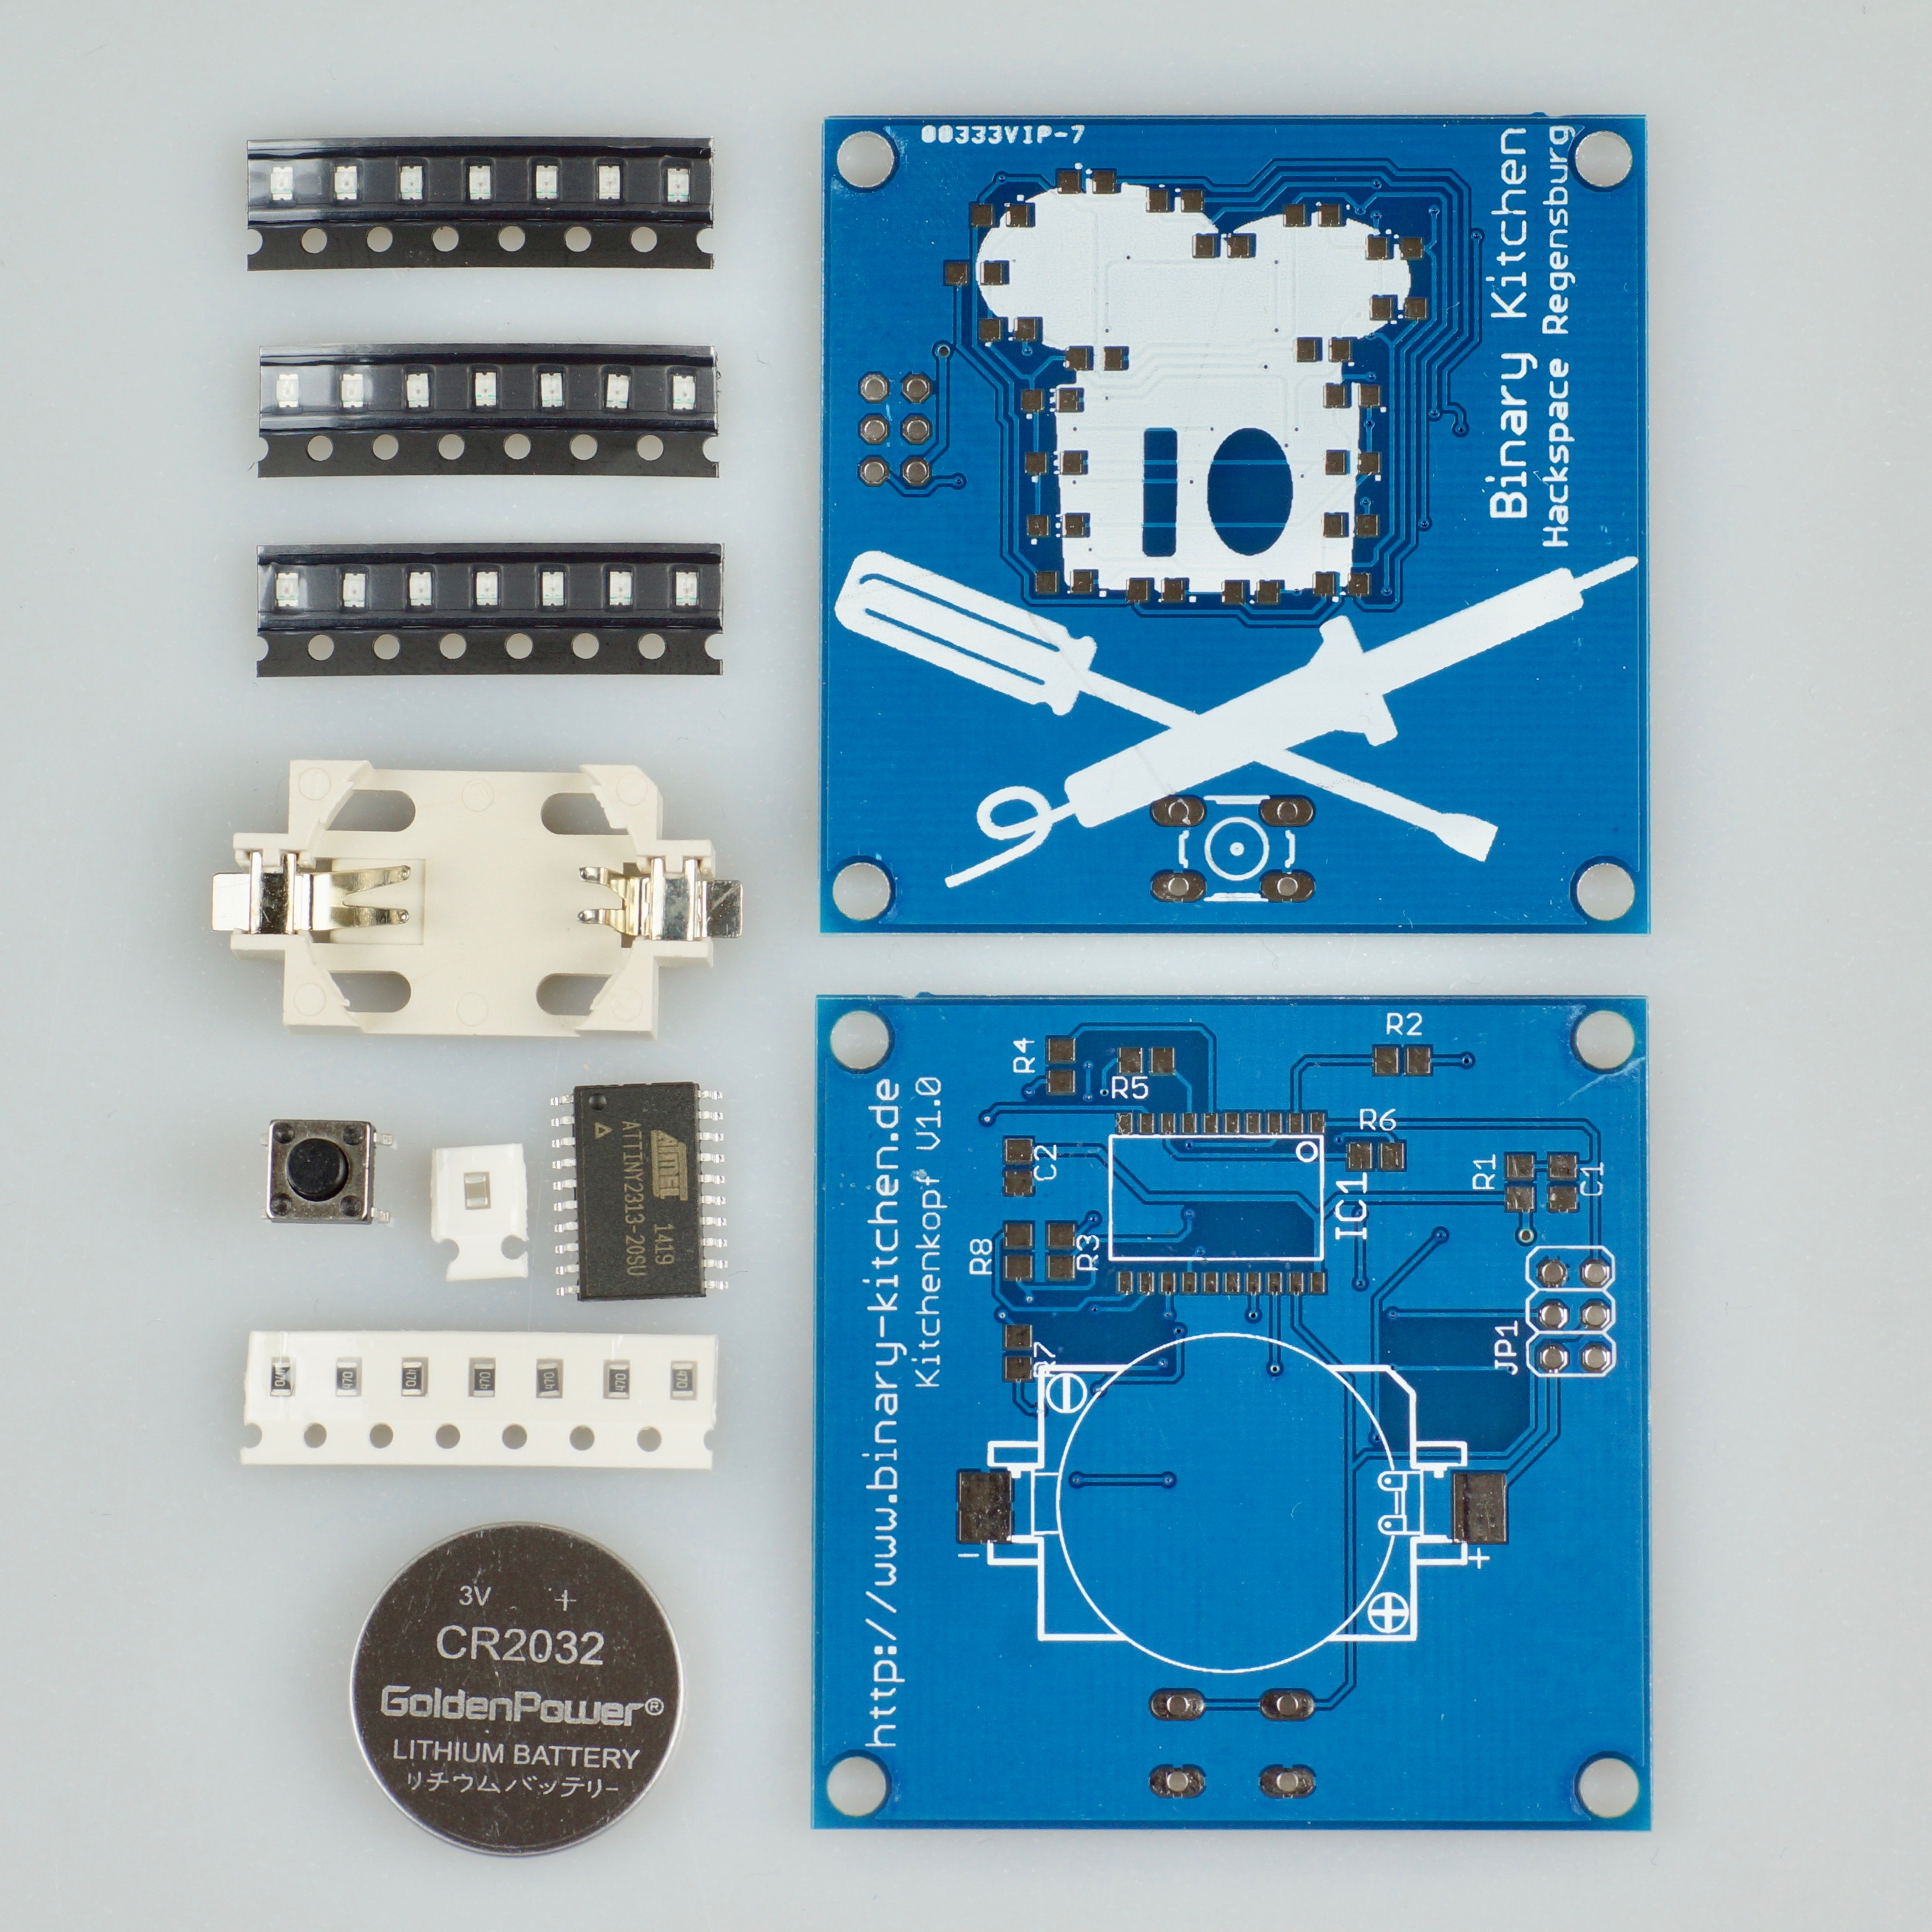
\includegraphics[width=0.95\columnwidth]{images/modified/DSC04829}
\par\end{flushright}%
\end{minipage}
\par\end{center}

\begin{center}
\vspace{5mm}
\rule[0.5ex]{0.9\columnwidth}{1pt}
\par\end{center}

\begin{center}
\begin{minipage}[t][1\totalheight][b]{0.59\columnwidth}%
\begin{enumerate}
\item L�tpads des IC1 mit Flussmittelgel aus Spritze bestreichen 
\item IC1 mit einem Klebeband aufnehmen. Klebeband sollte dabei nur die
H�lfte vom IC bedecken
\item Anschlie�end kann der IC mit Klebeband ausgerichtet und fixiert werden
\item Ausrichtung wichtig: Kleiner Punkt auf IC muss mit Punkt auf der Platine
links oben �bereinstimmen
\item Alle Beinchen mit L�tzinn auf der Platine aufl�ten
\item Anschlie�end kann Klebeband entfernt werden und die andere Seite befestigt
werden
\end{enumerate}
%
\end{minipage}\hspace{5mm}%
\begin{minipage}[t][1\totalheight][b]{0.3\columnwidth}%
\begin{flushright}
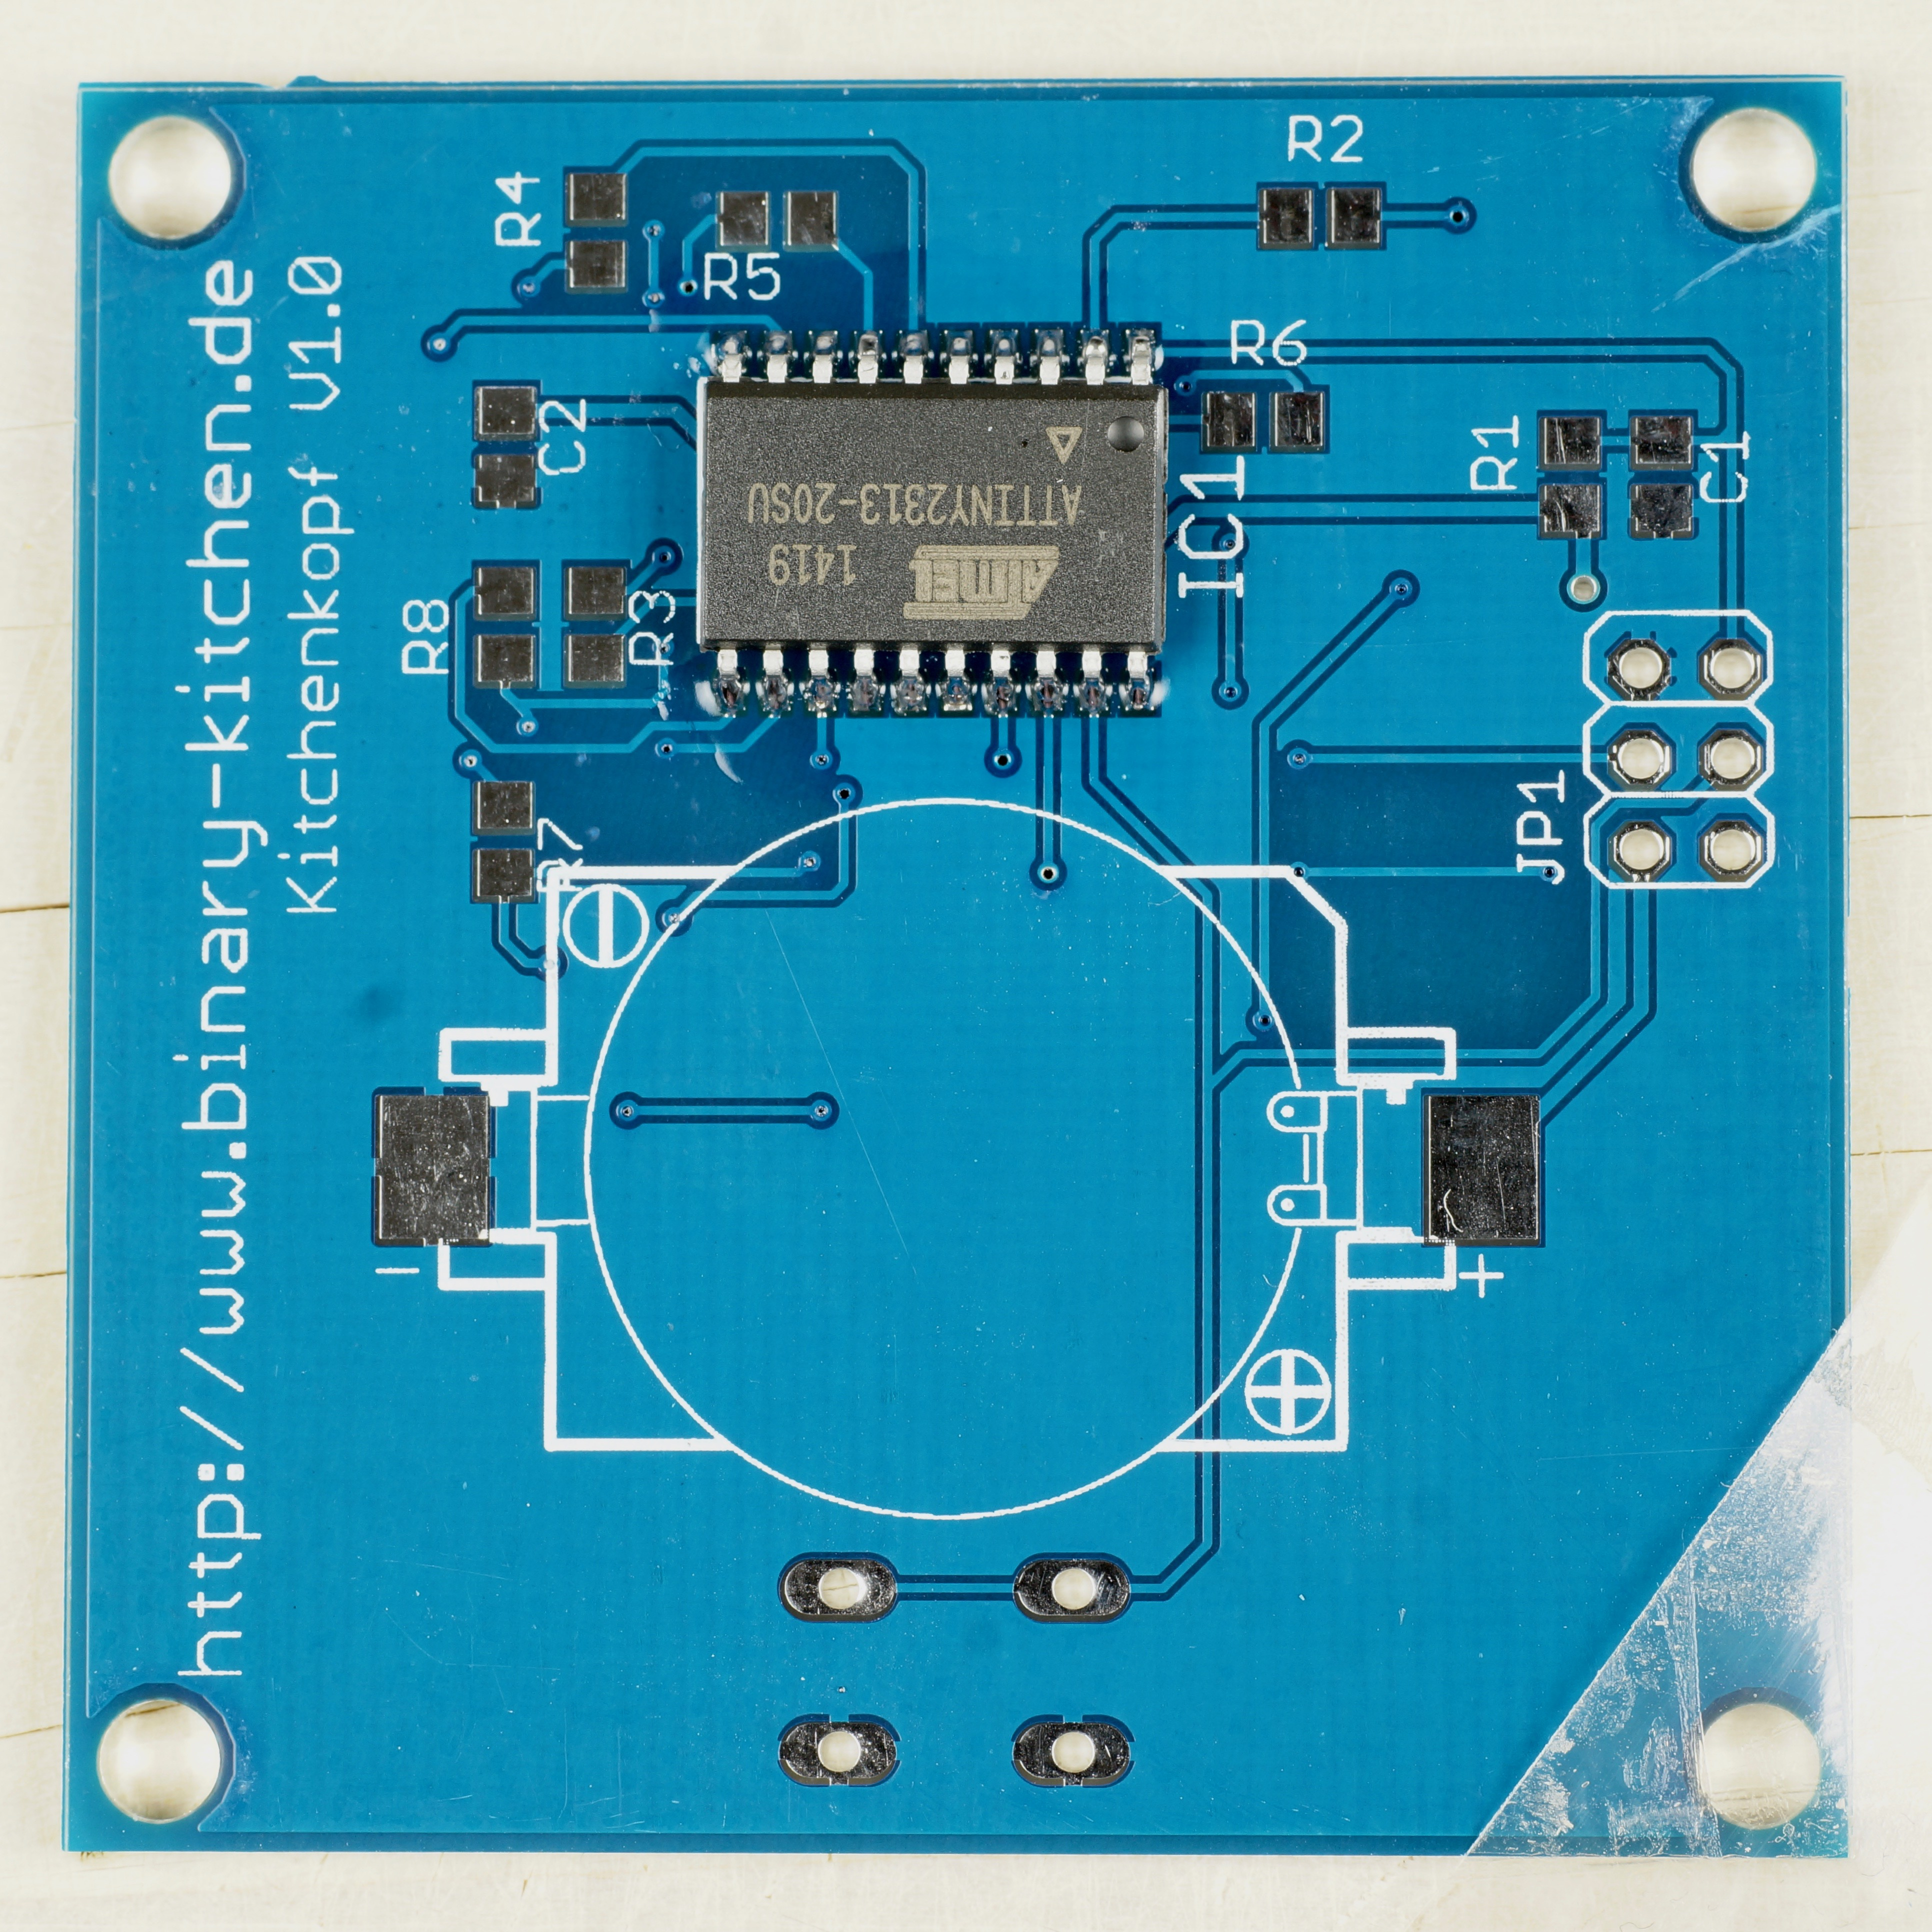
\includegraphics[width=0.95\columnwidth]{images/modified/DSC04831}
\par\end{flushright}%
\end{minipage}
\par\end{center}

\begin{center}
\vspace{5mm}
\rule[0.5ex]{0.9\columnwidth}{1pt}
\par\end{center}

\begin{center}
\begin{minipage}[t][1\totalheight][b]{0.59\columnwidth}%
\begin{enumerate}
\item Widerst�nde R2 bis R8 aufl�ten 
\item Dazu ein Pad verzinnen 
\item Anschlie�end Zinn aufheizen und den Widerstand seitlich mit der Pinzette
zuf�hren
\item Danach zweite Seite festl�ten
\end{enumerate}
%
\end{minipage}\hspace{5mm}%
\begin{minipage}[t][1\totalheight][b]{0.3\columnwidth}%
\begin{flushright}
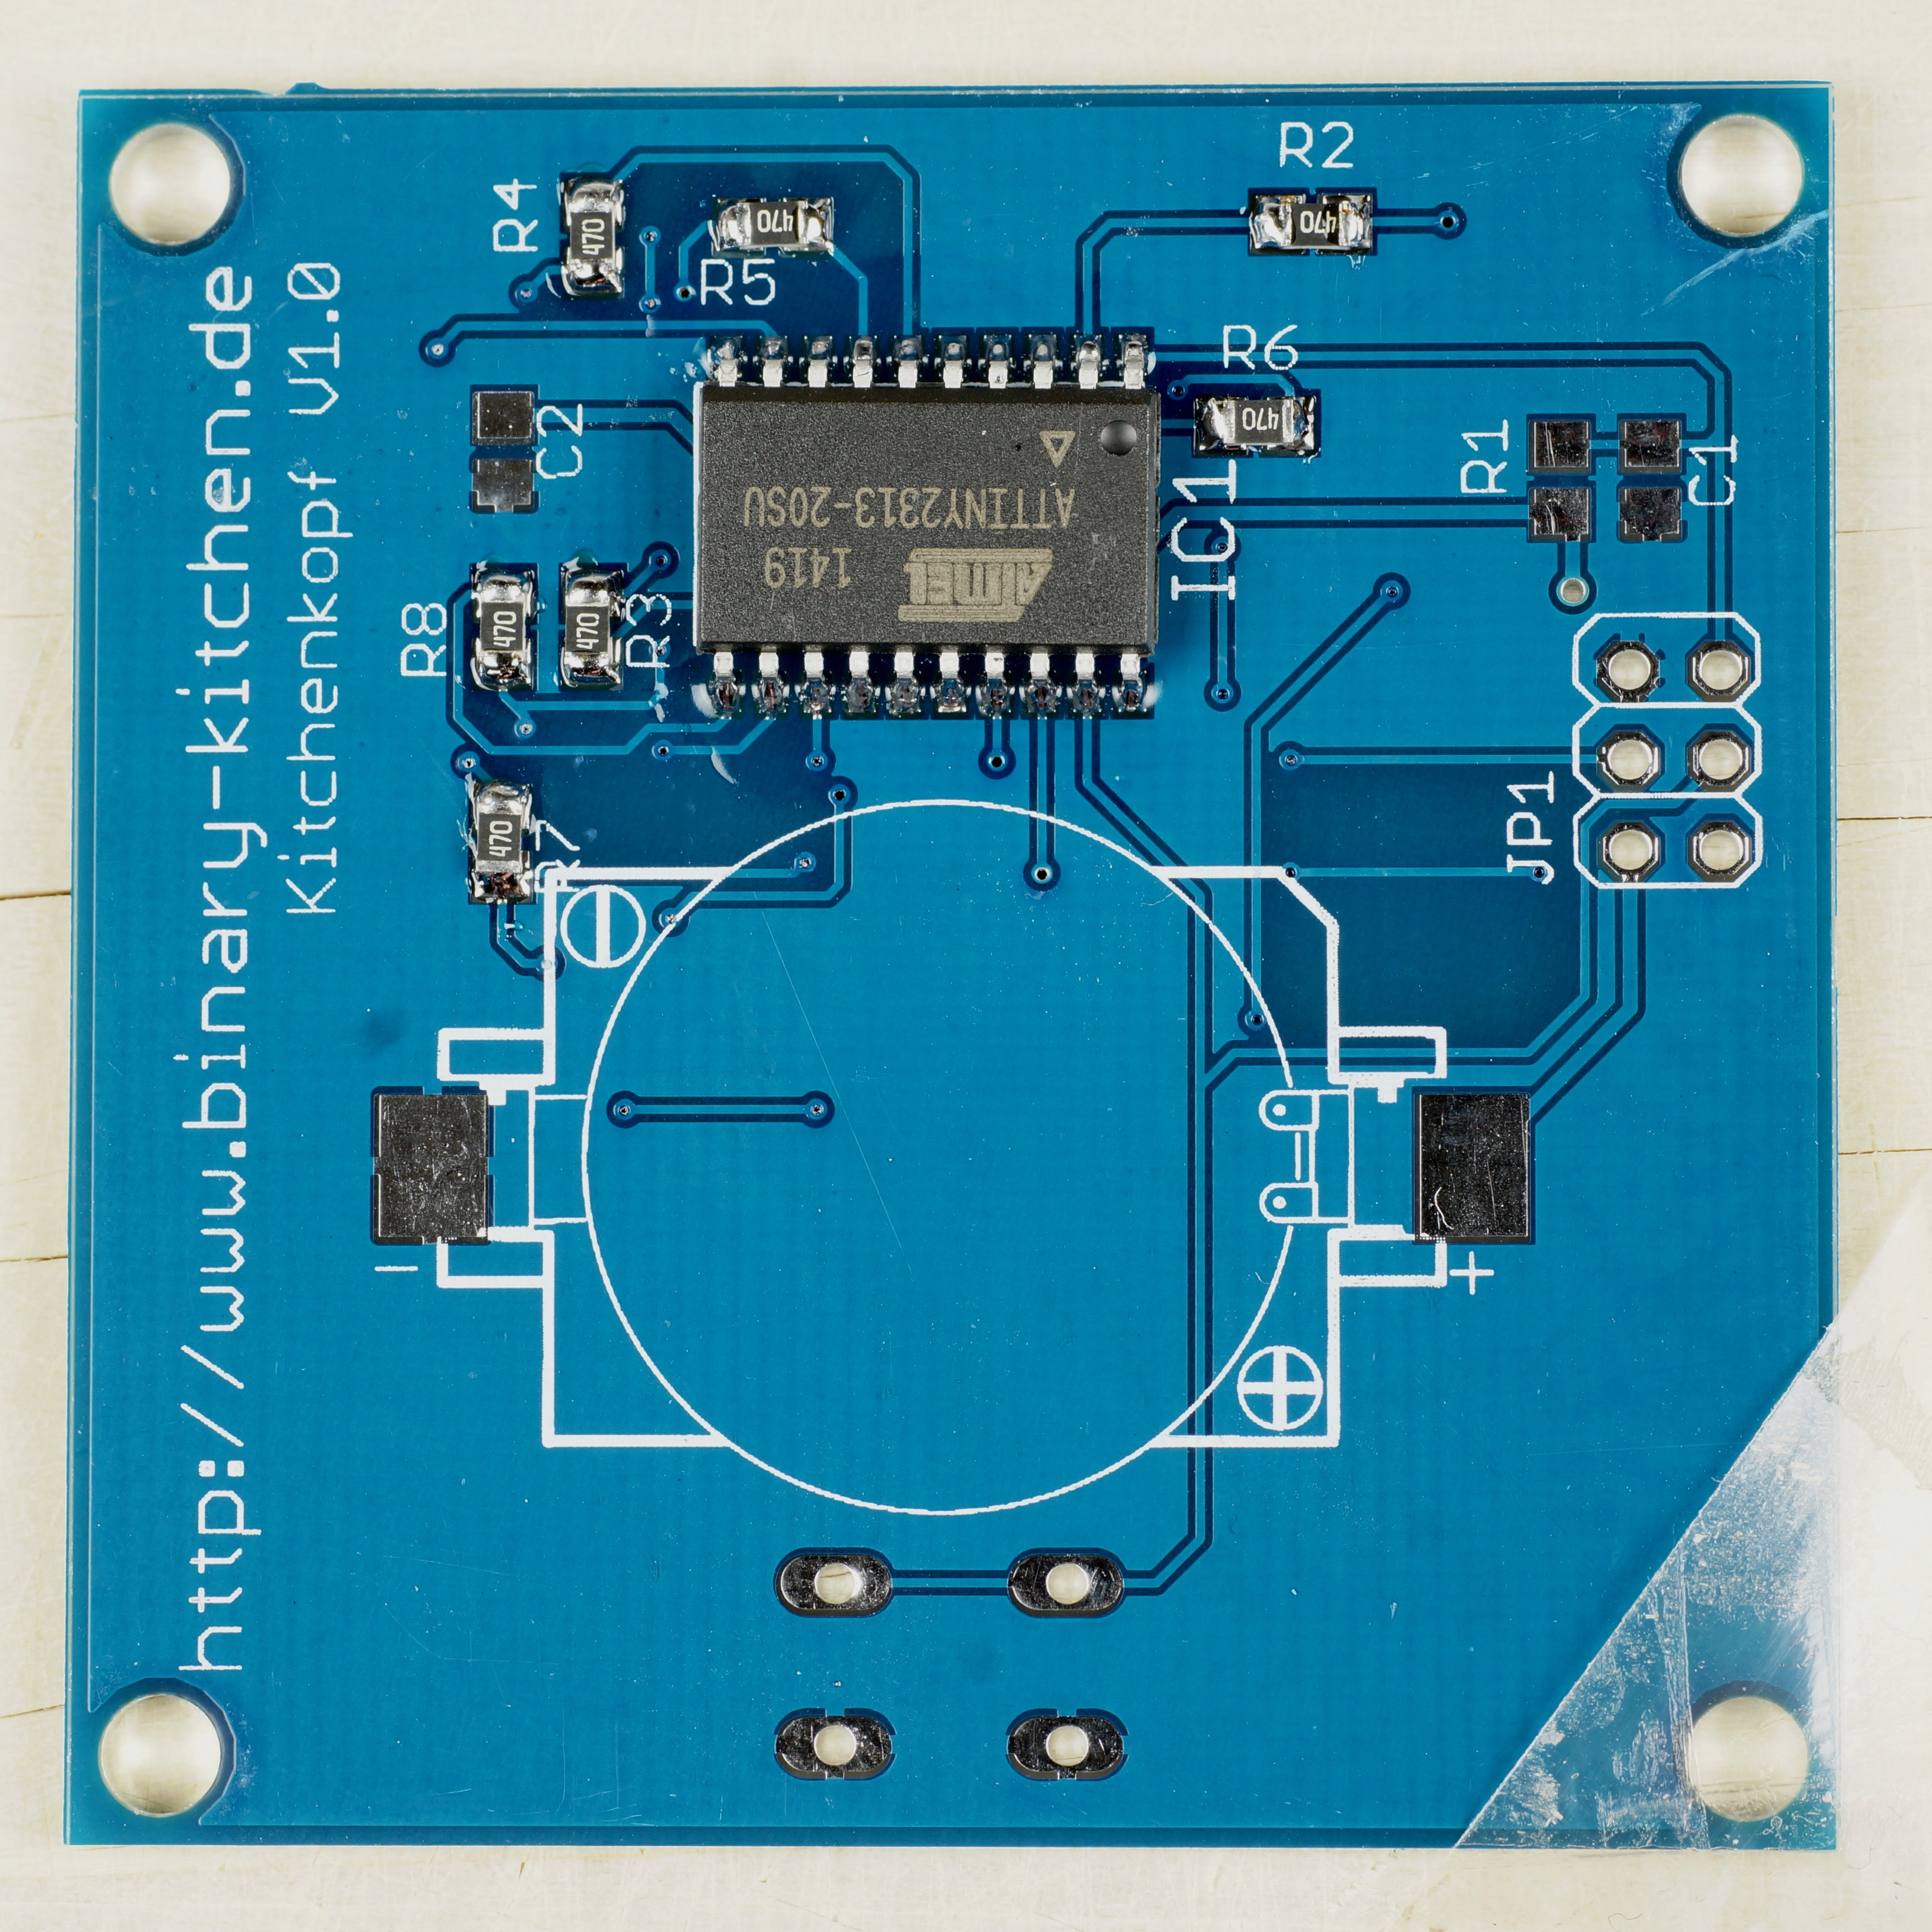
\includegraphics[width=0.95\columnwidth]{images/modified/DSC04832}
\par\end{flushright}%
\end{minipage}
\par\end{center}

\begin{center}
\vspace{5mm}
\pagebreak{}\rule[0.5ex]{0.9\columnwidth}{1pt}
\par\end{center}

\begin{center}
\begin{minipage}[t][1\totalheight][b]{0.59\columnwidth}%
\begin{enumerate}
\item Kondensator C2 mit der zuvor vorgestellten Technik aufl�ten
\end{enumerate}
%
\end{minipage}\hspace{5mm}%
\begin{minipage}[t][1\totalheight][b]{0.3\columnwidth}%
\begin{flushright}
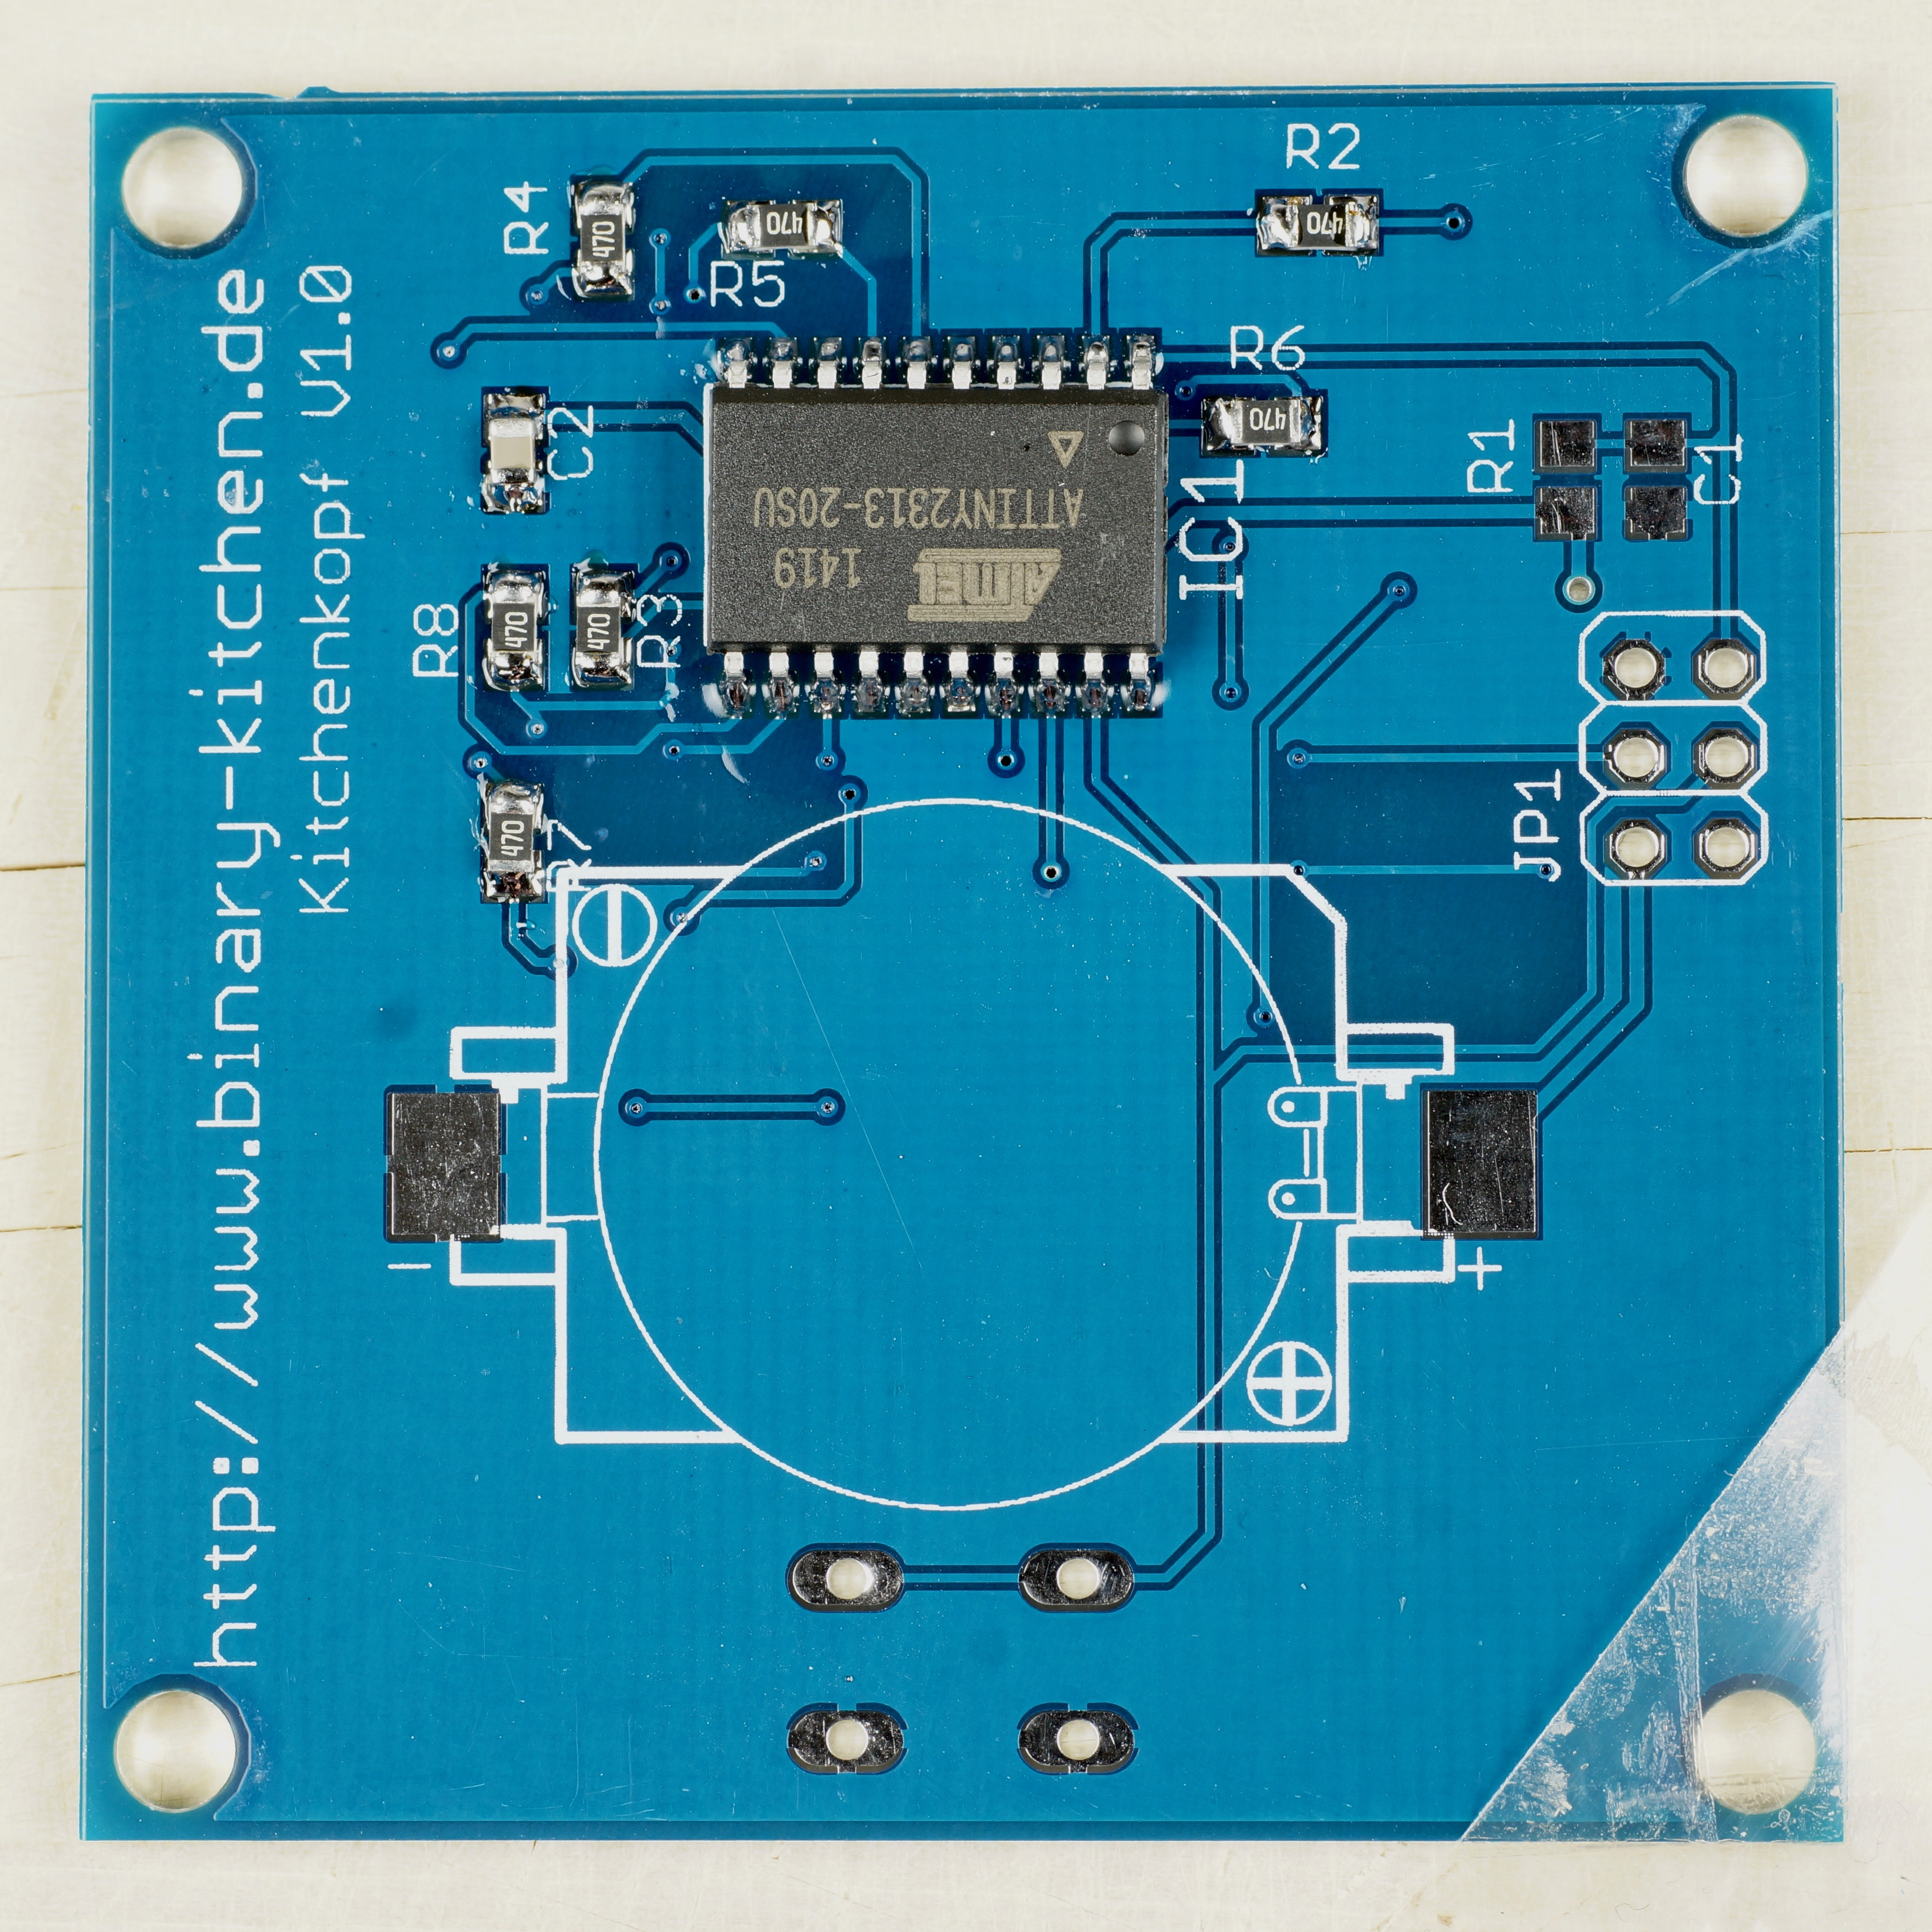
\includegraphics[width=0.95\columnwidth]{images/modified/DSC04833}
\par\end{flushright}%
\end{minipage}
\par\end{center}

\begin{center}
\vspace{5mm}
\rule[0.5ex]{0.9\columnwidth}{1pt} 
\par\end{center}

\begin{center}
\begin{minipage}[t][1\totalheight][b]{0.59\columnwidth}%
\begin{enumerate}
\item LEDs mit der zuvor vorgestellten Technik aufl�ten 
\item Dazu Platine umdrehen 
\item Ausrichtung wichtig: Auf der Platine sind Pfeile aufgedruckt. Auf
der LED ein T. Der Vertikale Strich des T muss auf die Seite der Pfeilspitze
zeigen
\end{enumerate}
\begin{center}

\includegraphics[height=7mm]{images/smd_led}
\par\end{center}%
\end{minipage}\hspace{5mm}%
\begin{minipage}[t][1\totalheight][b]{0.3\columnwidth}%
\begin{flushright}
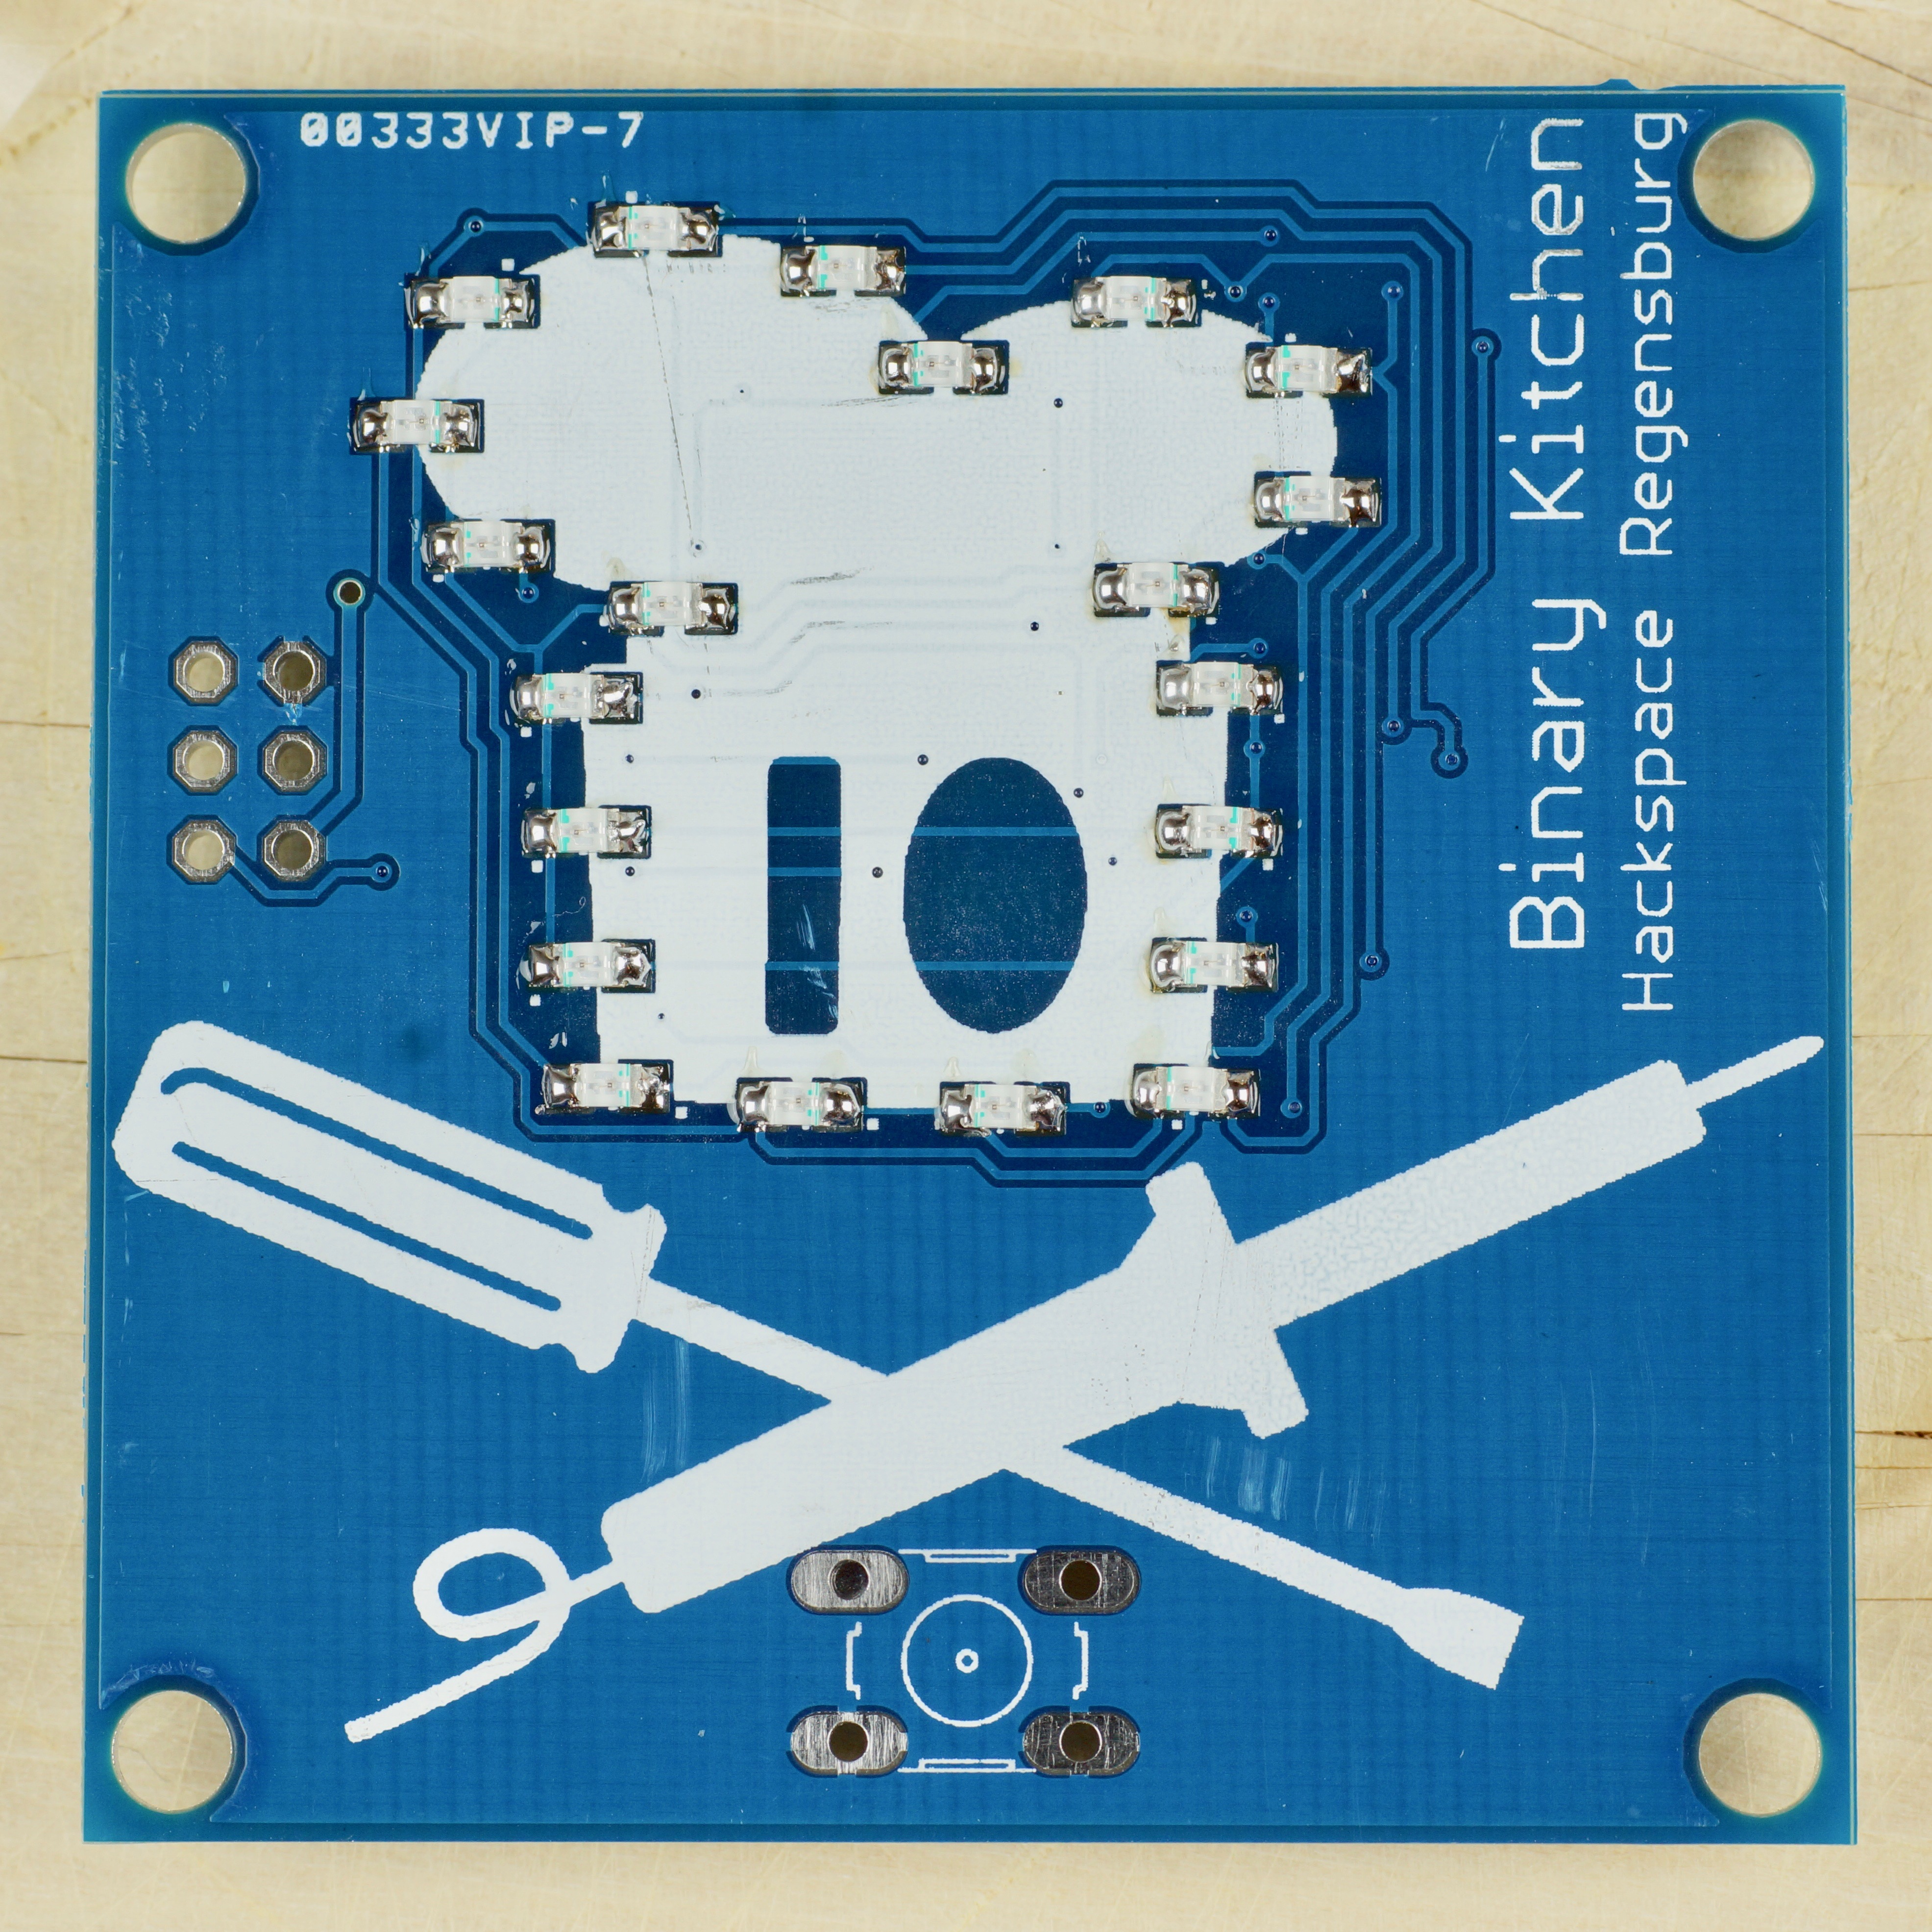
\includegraphics[width=0.95\columnwidth]{images/modified/DSC04834}
\par\end{flushright}%
\end{minipage}
\par\end{center}

\begin{center}
\vspace{5mm}
\rule[0.5ex]{0.9\columnwidth}{1pt}
\par\end{center}

\begin{center}
\begin{minipage}[t][1\totalheight][b]{0.59\columnwidth}%
\begin{enumerate}
\item Schalter S1 aufl�ten 
\item Tipp: Beinchen haben unterschiedliche Abst�nde. Es muss nichts verbogen
werden. Schalter passt exakt
\end{enumerate}
%
\end{minipage}\hspace{5mm}%
\begin{minipage}[t][1\totalheight][b]{0.3\columnwidth}%
\begin{flushright}
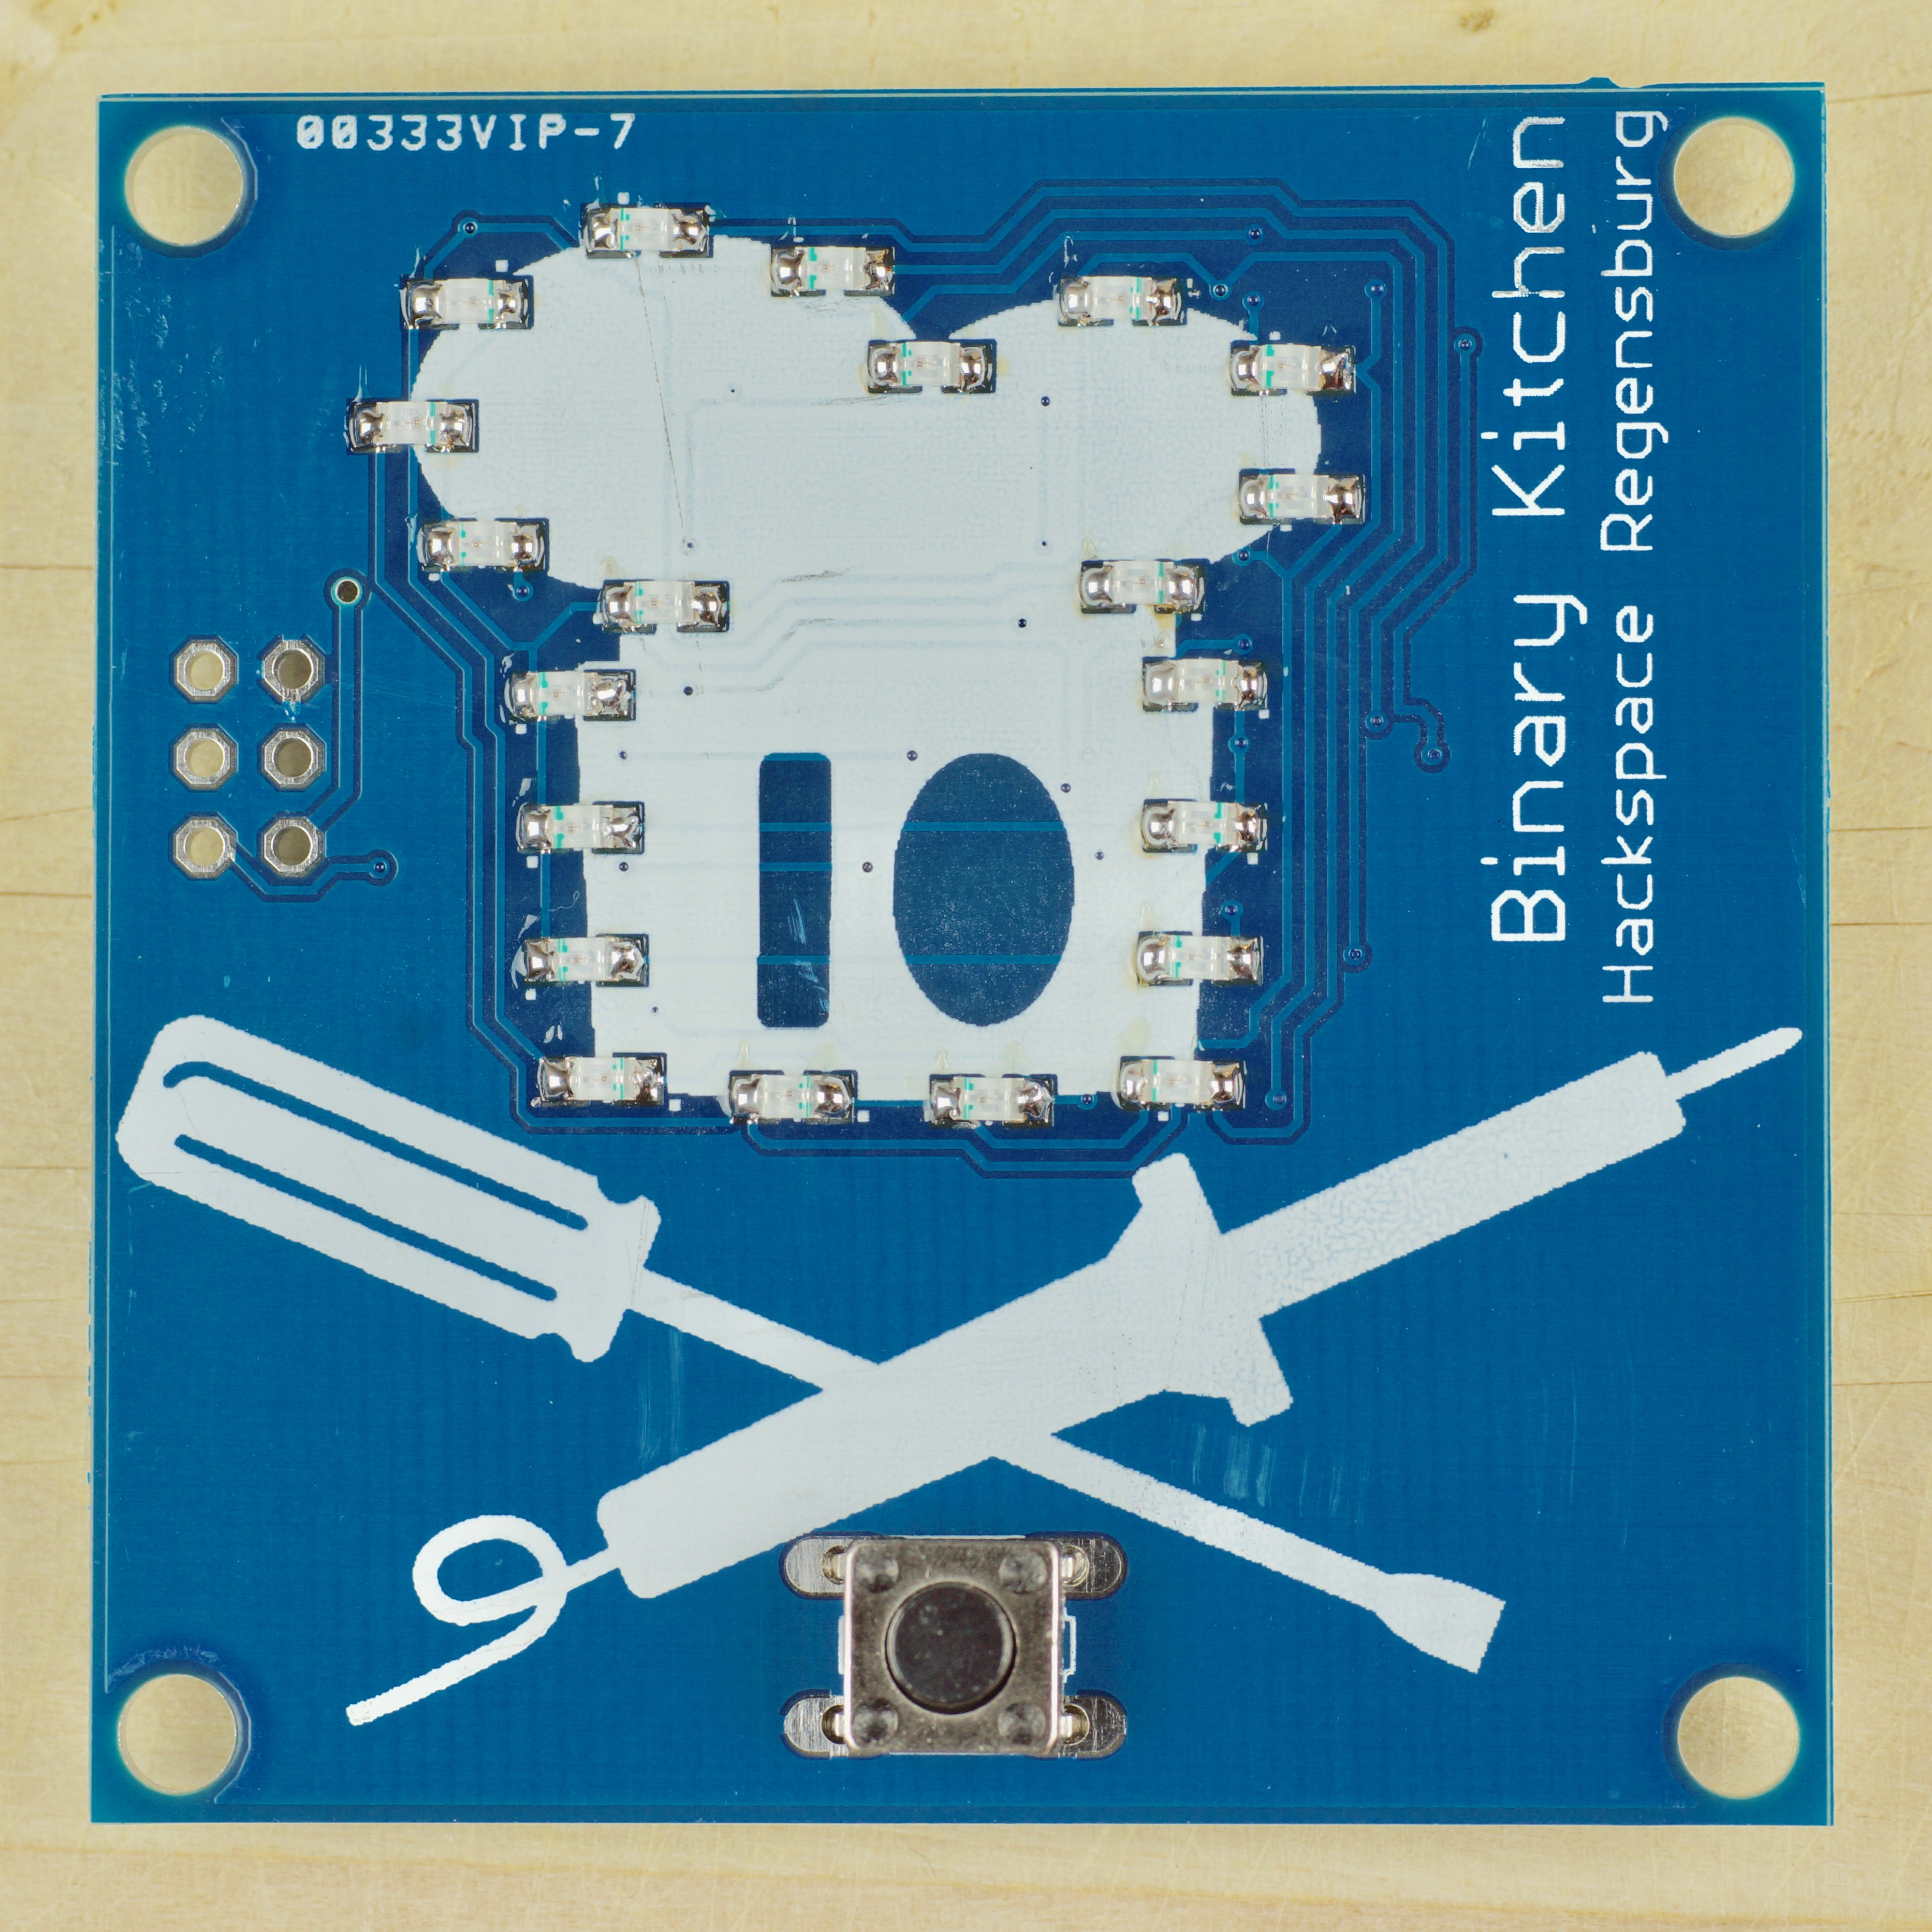
\includegraphics[width=0.95\columnwidth]{images/modified/DSC04835}
\par\end{flushright}%
\end{minipage}
\par\end{center}

\begin{center}
\vspace{5mm}
\pagebreak{}\rule[0.5ex]{0.9\columnwidth}{1pt}
\par\end{center}

\begin{center}
\begin{minipage}[t][1\totalheight][b]{0.59\columnwidth}%
\begin{enumerate}
\item Batteriehalter aufl�ten
\item Dazu Platine umdrehen
\item Batteriehalter und Platine haben aufgedrucktes Plus und Minus Symbol.
Dieses muss �bereinstimmen
\item Tipp: Beim Pluspol anfangen
\item Zuletzt Batterie einsetzen und Schalter bet�tigen
\end{enumerate}
%
\end{minipage}\hspace{5mm}%
\begin{minipage}[t][1\totalheight][b]{0.3\columnwidth}%
\begin{flushright}
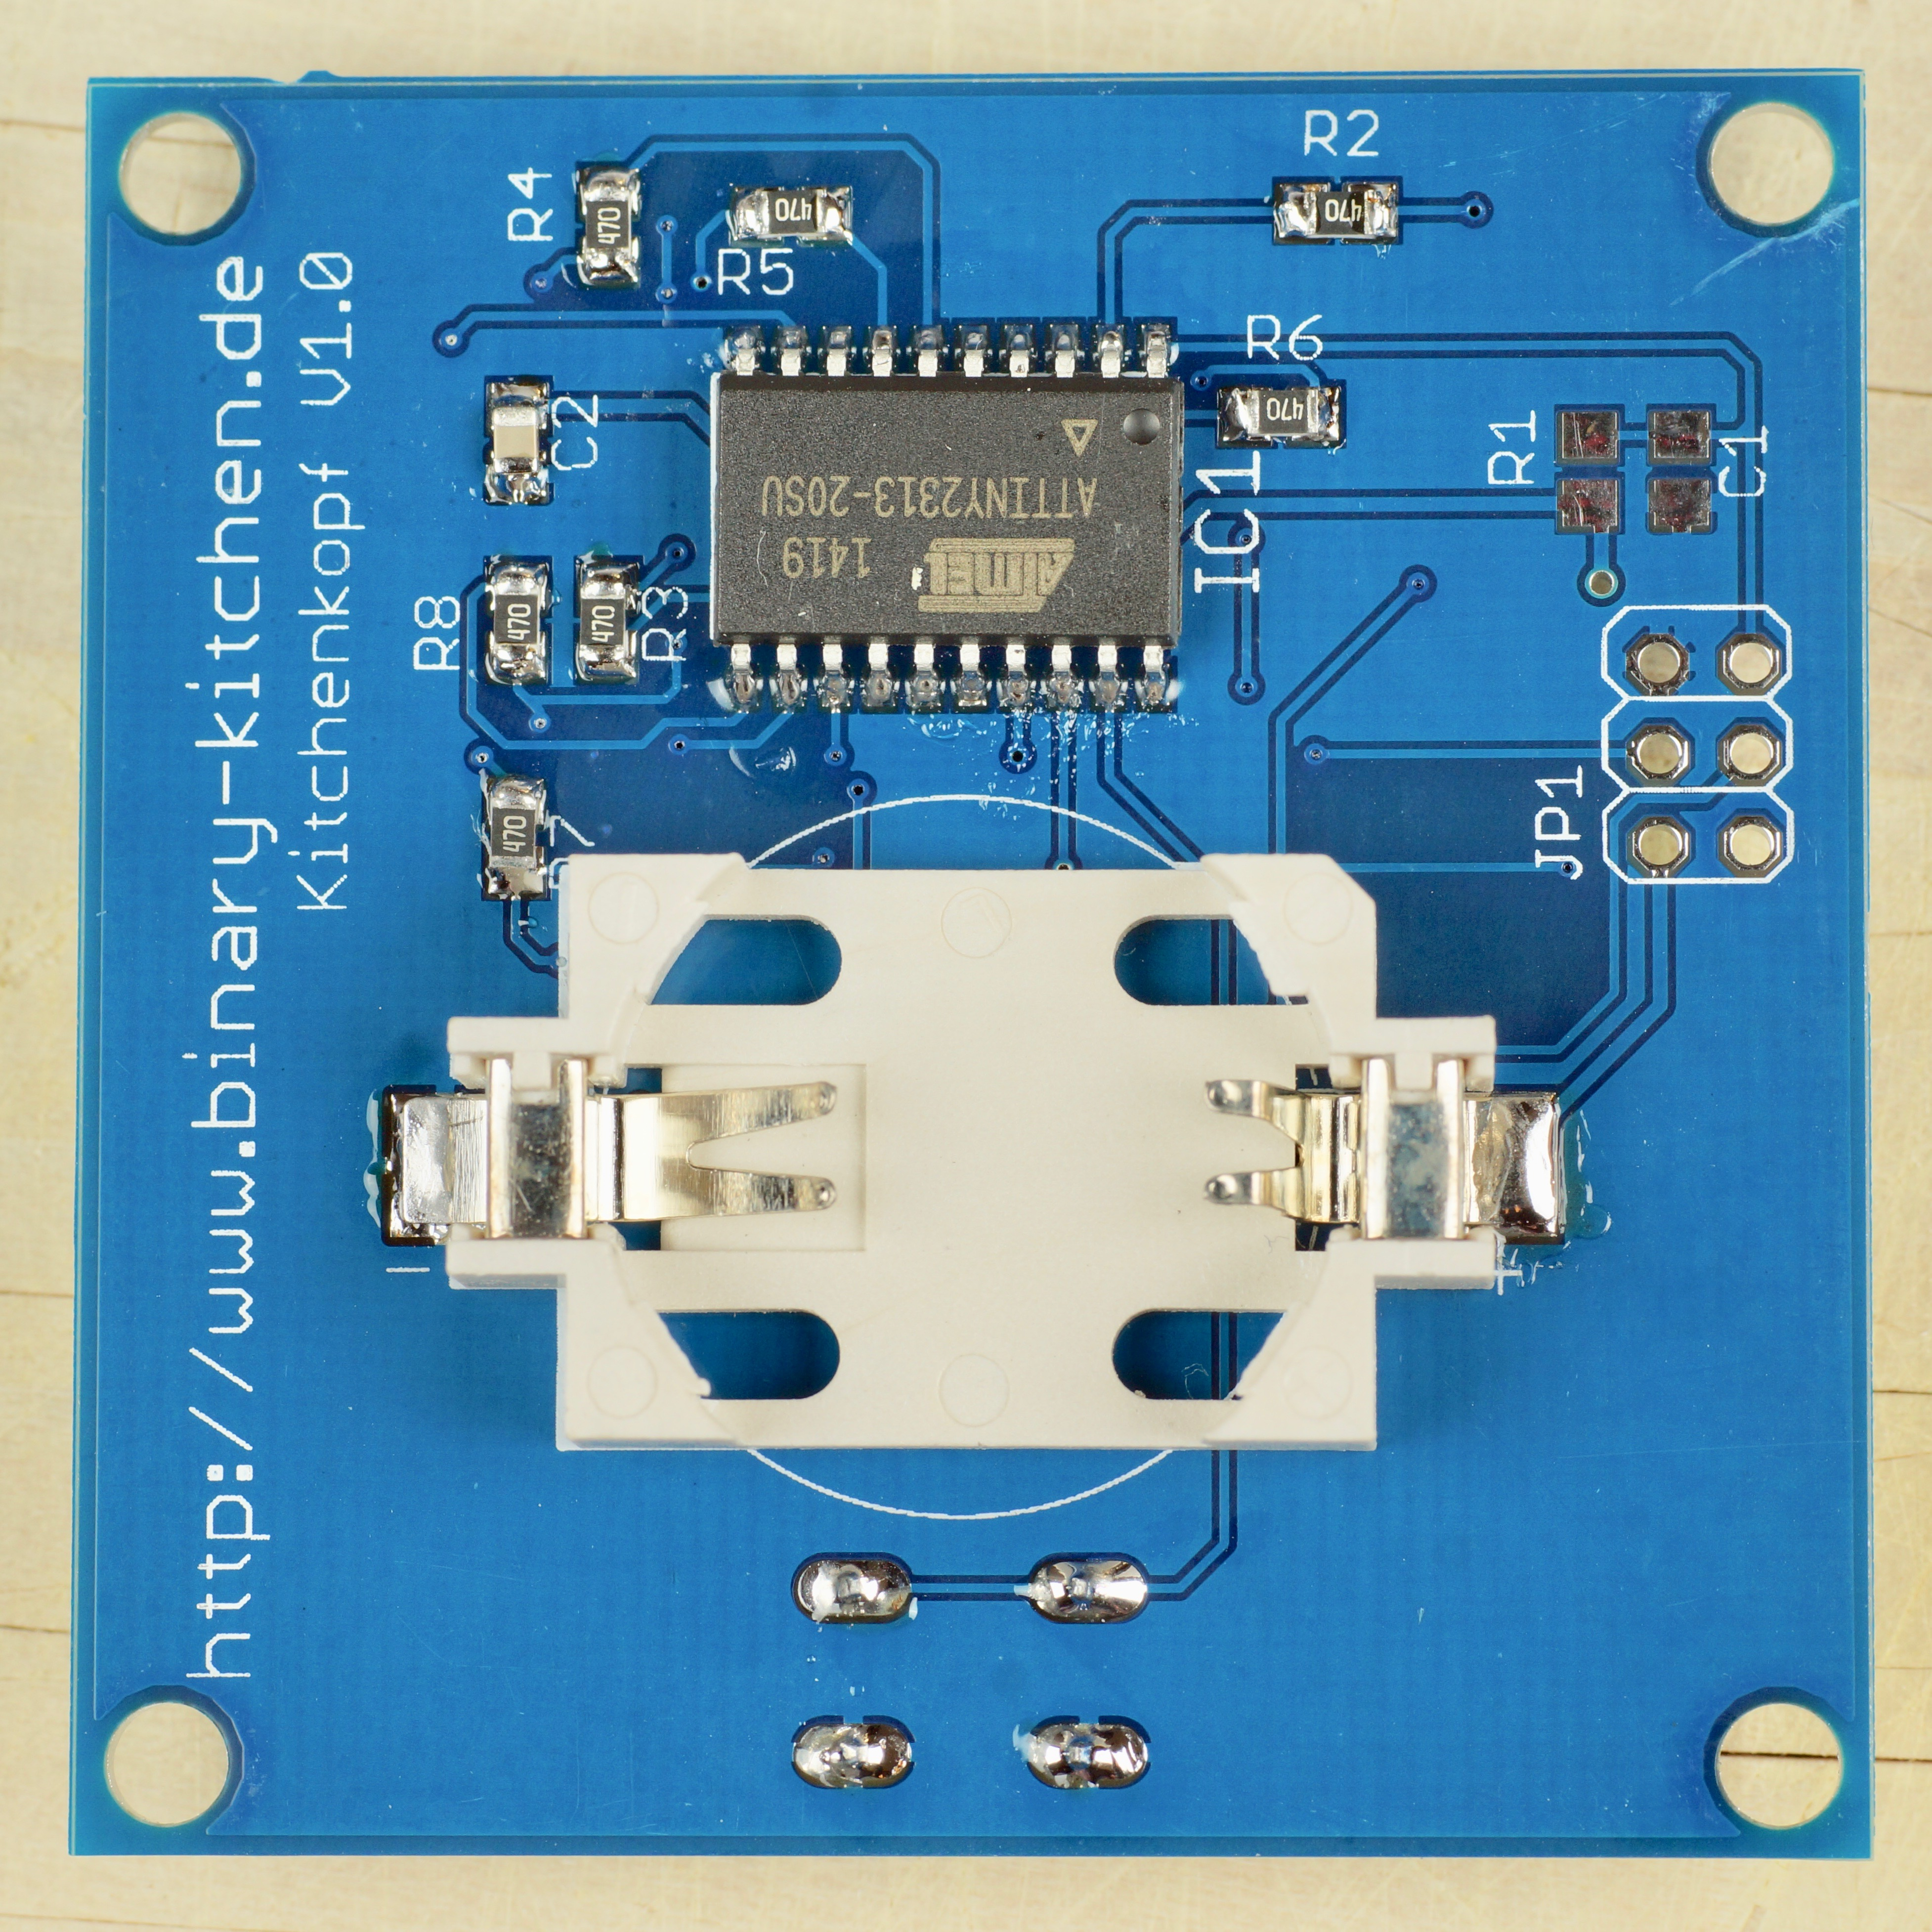
\includegraphics[width=0.95\columnwidth]{images/modified/DSC04836}
\par\end{flushright}%
\end{minipage}
\par\end{center}

\begin{center}
\vspace{5mm}
\rule[0.5ex]{0.9\columnwidth}{1pt}
\par\end{center}

\begin{center}
\begin{minipage}[t][1\totalheight][b]{0.3\columnwidth}%
\begin{center}
\includegraphics[bb=230bp 95bp 680bp 550bp,clip,width=0.95\columnwidth]{\string"images/Kitchenkopf-v1.1 - Top\string".pdf}
\par\end{center}%
\end{minipage}\hspace{5mm}%
\begin{minipage}[t][1\totalheight][b]{0.3\columnwidth}%
\begin{center}
\includegraphics[bb=200bp 100bp 650bp 550bp,clip,width=0.95\columnwidth]{\string"images/Kitchenkopf-v1.1 - Bottom\string".pdf}
\par\end{center}%
\end{minipage}
\par\end{center}
\end{document}
